\documentclass[11pt,a4paper]{article}
\usepackage[top=3cm, bottom=2cm, left=2cm, right=2cm]{geometry}
\usepackage[utf8]{inputenc}
\usepackage{amsmath, amsfonts, amssymb}
\usepackage{siunitx}
\usepackage[brazil]{babel}
\usepackage{graphicx}
\usepackage[margin=10pt,font={small, it},labelfont=bf, textfont=it]{caption}
\usepackage[dvipsnames, svgnames]{xcolor}
\DeclareCaptionFont{MediumOrchid}{\color[svgnames]{MediumOrchid}}
\usepackage[pdftex]{hyperref}
\usepackage{natbib}
\bibliographystyle{plainnat}
\bibpunct{\textcolor{MediumOrchid}{\textbf{[}}}{\textcolor{MediumOrchid}{\textbf{]}}}{,}{s}{}{}
\usepackage{color}
\usepackage{footnote}
\usepackage{setspace}
\usepackage{booktabs}
\usepackage{multirow}
\usepackage{subfigure}
\usepackage{fancyhdr}
\usepackage{leading}
\usepackage{indentfirst}
\usepackage{wrapfig}
\usepackage{mdframed}
\usepackage{etoolbox}
\usepackage[version=4]{mhchem}
\usepackage{enumitem}
\usepackage{caption}
\usepackage{titlesec}
\usepackage{tcolorbox}
\usepackage{tikz}
\usepackage{LobsterTwo}
\usepackage[T1]{fontenc}
\usepackage{fontspec}
\usepackage{txfonts}
\usepackage[bottom]{footmisc}
\tcbuselibrary{skins,breakable}
\sisetup{output-decimal-marker={.}}

\makeatletter
\def\footnoterule{\kern-3pt\color{MediumOrchid}\hrule\@width0.6\textwidth height 0.8pt\kern2.6pt}
\makeatother

\renewcommand{\footnotelayout}{\itshape\color{MediumOrchid}}

\AtBeginEnvironment{equation}{\fontsize{13}{16}\selectfont}


\titleformat{\section}{\LobsterTwo\huge\color{CarnationPink}}{\thesection.}{1em}{}
\titleformat{\subsection}{\LobsterTwo\huge\color{CarnationPink}}{\thesubsection}{1em}{}
\titleformat{\subsubsection}{\bf\LobsterTwo\Large\color{MediumOrchid}}{\thesubsubsection}{1em}{}


\DeclareCaptionLabelFormat{figuras}{\textcolor{DarkTurquoise}{Figura \arabic{figure}}}
\captionsetup[figure]{labelformat=figuras}

\makeatletter
\renewcommand\tagform@[1]{\maketag@@@{\color{CarnationPink}(#1)}}
\makeatother

\renewcommand{\theequation}{Eq. \arabic{equation}}
\renewcommand{\thefigure}{Fig. \arabic{figure}}
\renewcommand{\thesection}{\textcolor{CarnationPink}{\arabic{section}}}

\setlist[itemize]{label=\textcolor{CarnationPink}{$\blacksquare$}}

\setlist[enumerate]{label=\textcolor{CarnationPink}{\arabic*.}, align=left, leftmargin=1.5cm}


\newcounter{exemplo}

\NewDocumentEnvironment{exemplo}{ O{} }{%
\allowbreak
\setlength{\parindent}{0pt}
  \begin{mdframed}[
  leftline=true,
  topline=false,
  rightline=false,
  bottomline=false,
  linewidth=2pt,
  linecolor=CarnationPink,
  frametitlerule=false,
  frametitlefont=\LobsterTwo\large\color{CarnationPink},
  frametitle={\color{CarnationPink}\LobsterTwo\large #1},
  ]
}{%
  \end{mdframed}
}

\setlength{\fboxsep}{5pt}
\setlength{\fboxrule}{1.5pt}
\usepackage{float}
\renewcommand{\thefootnote}{\alph{footnote}}
\usepackage{url}
\hypersetup{
	colorlinks=true,
	linkcolor=DarkTurquoise,
	filecolor=DarkTurquoise,      
	urlcolor=DarkTurquoise,
	citecolor=DarkTurquoise,
	pdftitle={Especialista em Física da Radioterapia}
}
\pagestyle{fancy}
\fancyhf{}
\renewcommand{\headrulewidth}{0pt}
\rfoot{\thepage \\ \tiny{dalila.fismed@gmail.com}}

\title{\LobsterTwo\Huge{Dosimetria}}
\author{\LobsterTwo{Dosimetria Relativa}\nocite{*}}
\date{\LobsterTwo\textit{Dalila Mendonça}}
\begin{document}
	\maketitle


\section{Introdução}

	Existem dois objetivos principais na medida de dados de dosimetria relativa:
	
	\begin{enumerate}
		\item Confirmar a precisão da funcionalidade técnica do acelerador para produzir um feixe simétrico com energia correta e com output relativo conhecido, conforme especificado no teste aceite; e
		\item Caracterizar os feixes disponíveis provenientes do equipamento para serem inseridos no software de planejamento de tratamento (TPS).
	\end{enumerate}
	
\subsection*{Funcionalidade Técnica}

	A dosimetria relativa é muito sensível à mudanças técnicas no próprio acelerador. Por exemplo, alterações nas bobinas de direção (presentes na guia aceleradora) ou na câmara de ionização monitoras podem fazer com que a simetria do feixe se desvie acima dos limites especificados pelos testes de aceite e pelas recomendações da \textit{American Association of Physicists in Medicine (AAPM)}.

	A dosimetria relativa é usada durante os testes de comissionamento e aceite para ajustar os parâmetros técnicos do acelerador. Posteriormente, as medidas de dosimetria relativa são utilizadas como parte do QA periódico do acelerador para verificar o funcionamento preciso e consistente do acelerador. O TG-40 (antigo) e TG-142 (inclui novas tecnicas como IMRT e SRS/SBRT) fornecem tabelas detalhadas quanto as medidas de dosimetria relativa, frequências e tolerâncias recomendadas para a prática clínica em aceleradores lineares convencionais. AAPM TG-135 e TG-148 fornecem informações adicionais para CyberKnife e TomoTherapy, respectivamente.

\subsection{Caracterização do Feixe para o TPS}

	As medidas de dados adquiridos na dosimetria relativa durante o comissionamento são utilizadas como imput no TPS e nos cálculos secundários das unidades monitoras (MU). Portanto, é essencial que os dados sejam de alta qualidade, pois fornecem a base para o tratamento de milhares de pacientes durante a vida útil da máquina de tratamento. O conjunto de dados de dosimetria relativa obtidos durante o controle de qualidade anual serve a dois propósitos:
	
	\begin{enumerate}[label=\textcolor{CarnationPink}{\arabic*${}^\circ $}]
		\item É uma verificação mais rigorosa do desempenho do acelerador quando comparado às medidas dosimetria relativa mensais ou diárias; 
		\item Os dados da dosimetria anual são utilizados para confirmar que a máquina ainda é caracterizada com exatidão pelo conjunto de dados utilizados no TPS.
	\end{enumerate}
	
	Portanto, é importante utilizar os dados TPS (baseline) após o comissionamento como base para comparação. Por exemplo, se um valor medido era originalmente 2\% diferente do valor do TPS e mudou para uma diferença de 3.5\%  nos anos subsequentes, uma comparação cutilizando como baseline o valor medido originalmente ao invés dos valores utilizados no TPS, mostraria uma diferença de apenas 1.5\% e não os reais 3.5\%, o que oculta a real incompatibilidade  entre os dados do TPS e os dados do feixe.

	Os fornecedores do TPS geralmente fornecem uma lista de medidas de dosimetria relativa necessárias para o seu comissionamento. As principais abordagens para o comissionamento do TPS são:

	\begin{itemize}[label=\textcolor{CarnationPink}{$\blacktriangleright$}]
		\item O TPR pode requerer que sejam medidos um conjunto de dados de dosimetria relativa e que posteriormente sejam inseridos no TPS pelo usuário. Alguns desses tipos de TPS fornecem conjuntos de dados de feixe padrão para os aceleradores para fins de comparação, mas usam o conjunto de dados medidos para o planejamento do tratamento. Um exemplo dessa abordagem é o  TPS \textcolor{DarkTurquoise}{\textbf{MultiPlan}}		 para o CyberKnife.
		
		\item O TPS pode ser entregue juntamente com um conjunto de dados padrão para uma determinada máquina de tratamento. O conjunto de dados da dosimetria relativa medidos pelo usuário deve ser utilizado para verificar se a máquina é "suficientemente compatível" com o conjunto de dados padrão a ser utilizado para o planejamento do tratamento. Um exemplo dessa abordagem é o TPS \textcolor{DarkTurquoise}{\textbf{Eclipse}} da Varian. Atualmente, não há recomendações independentes do fabricante sobre a tolerância para a correspondência do conjunto de dados medido versus os dados padrão. Embora esse uso de dados de feixes pré-existentes não esteja de acordo com as recomendações do TG-106, ele segue uma prática clínica estabelecida para o TomoTherapy e Gamma Knife. Se essa abordagem for adotada, os dados fornecidos pelo fornecedor devem ser cuidadosamente comparados com os dados medidos e quaisquer desvios devem ser minuciosamente avaliados.
		
		\item Os dados medidos na dosimetria relativa são usados para gerar os parâmetros para um ou mais modelos de feixe. Exemplos dessa abordagem são os sistemas de planejamento Philips \textcolor{DarkTurquoise}{\textbf{Pinnacle}}, Elekta \textcolor{DarkTurquoise}{\textbf{XIO}} e RaySearch \textcolor{DarkTurquoise}{\textbf{RayStation}}. A modelagem de um feixe variando o tamanho de campo de um máximo 40 cm x 40 cm até um campo pequeno de 0.5 cm x 0.5 cm fornecendo um único conjunto de parâmetros pode levar a um comprometimento da precisão do modelo do feixe, que pode não ser aceitável na prática clínica. Nesses casos, pode ser prudente gerar dois modelos de feixe para a mesma energia  para corresponder à dosimetria relativa em todos os tamanhos de campo;
		
		\item O TPS pode fazer parte do sistema de entrega de tratamento e é reinstalado pelo fabricante. As medidas de dosimetria relativa são usadas apenas para verificar os dados gerados pelo fabricante. Um exemplo dessa abordagem é o sistema TomoTherapy e Leksell Gamma Knife (acredito que o Halcyon também faz parte desse time, pois não precisa de comissionamento, apenas o Aceite).
	\end{itemize}

	O rápido avanço da tecnologia também teve um impacto nas exigências para medidas de dosimetria relativa. As taxas de dose do acelerador aumentaram em um fator de 10 ou mais devido à melhorias no projeto do acelerador e à adoção de feixes sem filtro aplanador (FFF) em quase todos os sistemas de entrega de dose. A introdução da radioterapia de intensidade modulada (IMRT) e tratamento de arco modulado volumétrico (VMAT) aumentou a importância de medidas precisas da penumbra para modelar corretamente no TPS os gradientes de dose íngremes que ocorrem na borda do campo. As melhorias no projeto do colimador multilâminas (MLC) reduziram a largura da lâmina para 2.5 mm em alguns casos, permitindo o tratamento de alvos tão pequenos quanto 5 mm usando a ``regra de ouro'' de 2 x a largura mínima da lâmina. Esse desenvolvimento requer o uso de técnicas de dosimetria relativa de campos pequenos, que anteriormente eram restritas à dispositivos de radiocirurgia estereotáxica/radioterapia corporal estereotáxica (SRS/SBRT). O aumento do uso de regimes de tratamento com técnicas de SRS, SBRT e hipofracionado aumentou as demandas na precisão da dosimetria relativa, porque o impacto nos erros sistemáticos introduzidos por incertezas na dosimetria relativa na precisão da entrega do plano clínico é maior em comparação com os esquemas convencionais de fracionamento. O TG-106 define um “campo pequeno” como qualquer campo igual ou inferior a um campo quadrado equivalente de 4 cm x 4 cm, enquanto que um “Campo muito pequeno” denota campos iguais ou menores a um campo quadrado equivalente de 2 cm x 2 cm.

\section{Equipamento de Comissionamento}

\subsection*{Tanque de Água}

	Dever ser utilizado um Phantom de água com as seguintes características:

	\begin{enumerate}
		\item Dimensões apropriadas para medir o maior tamanho de campo necessário, além de vários centímetros de profundidade/largura adicionais para criar retroespalhamento nas bordas do campo;
		\item Um suporte para o phantom que permite o seu alinhamento;
		\item Eixos de movimento 2D ou 3D que podem ser ajustados de forma que o detector se mova paralelamente à superfície da água;
		\item Uma função automatizada de eixo central (CAX) para compensar pequenos desvios do CAX do feixe no movimento vertical do detector;
	\end{enumerate}

	Além destes grandes tanques de água tradicionais utilizados no comissionamento, existem  tanques pequenos de água disponíveis que são especializados para medir a razão tecido-phantom (TPR) em campos pequenos ou realizar os QAs mensais.

	Para medidas de dosimetria mensal e especialmente diárias, são usados phantoms sólidos no lugar de tanques de água. Esses materiais devem ter uma densidade eletrônica o mais próxima possível da água ou do tecido muscular. Como esses materiais não são condutores elétricos, existe a preocupação de que o buildup de carga possa levar a leituras errôneas se forem usados tempos de medidas prolongados ou doses muito altas. \textcolor{MediumOrchid}{\textbf{Obs:} Como, principalmente na América do Norte, é utilizado o TG-51 nas dosimetrias mensais e, como o próprio TG-142 e o Guideline 8 da AAMP sugere, a dosimetria mensal pode ser feita utilizando placas de água sólida para confirmar a constância do feixe, verificando se a calibração continua dentro dos limites mensais.  Portanto, não é necessário utilizar um tanque de água na dosimetria mensal caso a calibração anual seja realizada de acordo com o protocolo do TG-51. Nós aqui do BR utilizamos o TRS-398, então, vamos fazer na água pq não falaram nada da gente hehehehe.}

\subsection*{Dosímetros 1D}

	Os dosímetros que medem uma dose em um volume relativamente pequeno (aproximadamente dose pontual) se enquadram em duas categorias:

	\begin{enumerate}
		\item Detectores de medida única que precisam ser processados para leitura.\textcolor{MediumOrchid}{\textbf{Exemplo:}}TLD, OSLD, transistor de efeito de campo de semicondutor de óxido metálico (MOSFET) e pastilhas de alanina. 
		\item Detectores que podem ser operados com leitura contínua para fazer leituras múltiplas em um local ou leituras consecutivas ao longo de uma trajetória. \textcolor{MediumOrchid}{\textbf{Exemplo:}} câmaras de ionização, diodos e detectores de diamante.
	\end{enumerate}


	As câmaras de ionização têm sido o padrão-ouro para medir dados de dosimetria relativa. Para campos de até 4 cm x 4 cm, as câmaras do tipo Farmer são o padrão-ouro para medidas de dose pontual. Em campos menores que 4 cm x 4 cm, especialmente em feixes FFF, o comprimento da câmara Farmer leva ao efeito de média de volume, o que reduz a dose pontual medida em comparação com a dose pontual real. Portanto, câmaras de ionização de volume pequeno, de aproximadamente 0.006 \unit{cm^3} devem ser utilizadas para campos pequenos. Várias questões físicas pertinentes a câmaras pequenas precisam ser estudadas antes de usá-las na dosimetria relativa: relação sinal-ruído, corrente de fuga, efeito de haste aumentado em relação ao tamanho da câmara, dependência energética aumentada e estabilidade da corrente. Alguns autores recomendam que as câmaras de ionização não sejam usadas para levantamento do perfil do feixe na dosimetria relativa.

	Os diodos são cada vez mais usados para complementar as câmaras de ionização, especialmente para medidas de dosimetria em campos pequenos. Diodos estereotáxicos dedicados, com tamanho de diâmetros de detector ativo de 0.8 mm a 1 mm permitem medidas de penumbra altamente precisas. Os diodos estão disponíveis como modelos blindados e não blindados; os modelos não blindados são mais sensíveis às componentes de baixa energia do feixe de radiação. Os diodos também são úteis para medir a PDP em um feixe de elétrons (uma vez que nenhuma conversão da curva de ionização para dose é necessária), mas eles não devem ser usados para medidas de PDP em um feixe de fótons devido à sua resposta de energética. Os detectores de diamante são muito semelhantes aos diodos tanto em tamanho quanto em suas características físicas como detectores semicondutores de estado sólido. A principal razão pela qual os detectores de diamante não foram generalizadamente adotados em uso clínico, em comparação com os diodos é devido a sua limitada disponibilidade comercial e seu preço. Outro tipo de detector de estado sólido, o MOSFET, não é útil para comissionamento devido ao seu curto tempo de vida.


	As medidas de dose pontual para obter os fatores de output também podem ser realizadas usando pastilhas de gel de alanina. O gel de alanina é quase equivalente à água e, portanto, pode ser usado em uma ampla gama de energias de raios-x. Assim como os dosímetros termoluminescentes (TLD) e os dosímetros de luminescência estimulada opticamente (OSLD), as pastilhas de alanina podem ser utilizadas para verificação de dosimétrica em laboratórios de dosimetria credenciados. A incerteza do detector de alanina é da ordem de 1.7\%

	Os detectores TLD e OSLD são usados pelos laboratórios de dosimetria credenciados pelo Accredited Dosimetry Calibration Laboratory (ADCL), pelo Imaging and Radiation Oncology Core (IROC) QA Center Houston e pela IAEA para verificação dosimétrica da calibração do feixe. Devido ao seu pequeno tamanho, eles também podem ser usados para medir fatores de output. A incerteza de medição para um sistema TLD/OSLD bem mantido e calibrado é de cerca de 3\%. Embora TLDs e OSLDs normalmente não sejam usados para medidas de comissionamento por si só, eles podem ser muito úteis como um sistema interno de dosimetria secundária para realizar uma verificação cruzada das calibrações de dosimetria de referência em medidas de fator de output em campos pequenos. O TG-191 fornece recomendações sobre o uso do OSLD para dosimetria. 

\subsection*{Dosímetros 2D e 3D}

	Os filmes radiográficos e radiocrômicos são os dosímetros de maior resolução 2D disponíveis. O TG-69 contém informações e recomendações sobre o uso de filme radiográfico. Como muitas aplicações das imagens realizadas filme foram substituídas por dispositivos de imagem de portal eletrônico (EPIDs), a manutenção de uma sala escura e um processador de filme para processamento de filme radiográfico aumentou o custo do controle de qualidade com filme radiográfico e a maioria das instituições não possui mais um processador em funcionamento. A disponibilidade de filmes radiográficos está se tornando cada vez mais limitada. Portanto, muitos físicos têm ou estão em processo de mudança de medidas de dosimetria relativa para filme radiocrômico.

	O TG-235 descreve as propriedades, uso e manuseio de filmes radiocrômicos para dosimetria clínica. O filme radiocrômico oferece a vantagem distinta de fácil manuseio, uma vez que a exposição curta à luz visível é aceitável e o filme pode ser facilmente cortado no tamanho e formato desejados. As desvantagens incluem custo relativamente alto, não uniformidade de resposta ao longo do filme causada pela não uniformidade da luz do scanner nas bordas do escaneamento e dependência da dose com base na orientação do filme. A dosimetria precisa usando filme radiocrômico requer as seguintes etapas:

	\begin{enumerate}[label=\textcolor{CarnationPink}{\arabic*${}^\circ $}]
		\item Transporte, manuseio e armazenamento dentro da faixa de temperatura recomendada pelo fabricante e protegido de fontes de luz (em excesso ou longos períodos);
		
		\item Um scanner de mesa de alta qualidade capaz de digitalizar na faixa espectral apropriada definida pelo filme. O comissionamento inclui estabelecer a área de mesma intensidade de luz para evitar a introdução de desvios sistemáticos devido a mudanças no campo de luz nas bordas da área de escaneamento;
		
		\item Estabelecer a densidade de fundo para cada lote de filme, digitalizando um filme não irradiado. No entanto, pode ser utilizada uma técnica de canal de três cores que pode eliminar a necessidade de estabelecer a densidade de fundo;
		
		\item Para cada lote de filme, deve ser realizado o escaneamento do filme onde foi realizada uma irradiação escalonada ou irradiação  múltipla para estabelecer a curva de densidade óptica;
		
		\item O filme deve ser digitalizado em um intervalo de tempo definido após a irradiação para evitar a introdução de erros sistemáticos devido à mudança de cor pós-irradiação;
	\end{enumerate}

	Foi reportado um protocolo para o uso de filme radiocrômico que depende da resposta relativa de três canais de cores, minimizando assim os efeitos das variações e artefatos do filme e eliminando a necessidade de escanear o filme antes da irradiação.

	Uma alternativa ao filme são as matrizes de detectores 2D, que consistem em câmaras ou diodos dispostos em um padrão simétrico. Eles são frequentemente usados para medidas de dosimetria relativa como parte de um controle de qualidade diário ou mensal para verificar a planura e a simetria do campo, bem como os fatores filtro. Devido à distância física entre os detectores, os arrays 2D ainda não têm resolução para medir com precisão a penumbra do feixe para dosimetria relativa durante o comissionamento. No entanto, eles podem ser usados no comissionamento de entregas dinâmicas, como o comissionamento de filtros dinâmicos.

	O uso de dosimetria via EPID e cintiladores plásticos é um desenvolvimento mais recente na dosimetria 2D, prometendo resolver o problema de resolução de outras matrizes 2D. A dosimetria EPID é neste momento a tecnologia mais desenvolvida desses dois tipos de detectores. Os EPIDs disponíveis comercialmente geralmente têm tamanhos de pixel de cerca de 0.4 mm, com áreas ativas de até 40 \unit{cm^2}. Embora o uso de EPID esteja sendo desenvolvido ativamente e usado para dosimetria no QA de IMRT pré-tratamento, seu uso em dosimetria relativa não foi estabelecido. As razões para isso são problemas com o retroespalhamento do braço de suporte, a sensibilidade do pixel e a falta ou limitada flexibilidade da posição do painel para alterar a SSD.

	A dosimetria 3D pode ser realizada usando géis poliméricos. No entanto, não existem recomendações da sociedade sobre o uso de géis poliméricos para medidas de dosimetria relativa. Uma vez que o detector tem potencial para aquisição rápida de múltiplos parâmetros de feixe (OF (fator de output), PDP e OARs  em uma exposição), pode-se esperar um aumento no seu uso para medidas de QA de dosimetria relativa rotineiras.

	A \ref{fig:dosimetrosDosimetriaRelativa} mostra os principais dosímetros utilizados em dosimetria e suas principais aplicações. O sinal de $+$ indica o quanto aquele dosímetro é indicado para dado o parâmetro, $-$ indica que o dosímetro não é indicado para o parâmetro. A câmara estereotáxica se refere às câmaras de ionização com volumes sensíveis muito pequenos, utilizados na dosimetria de campos pequenos.

	\begin{figure}[h]
		\centering
		\fcolorbox{DarkTurquoise}{white}{%
			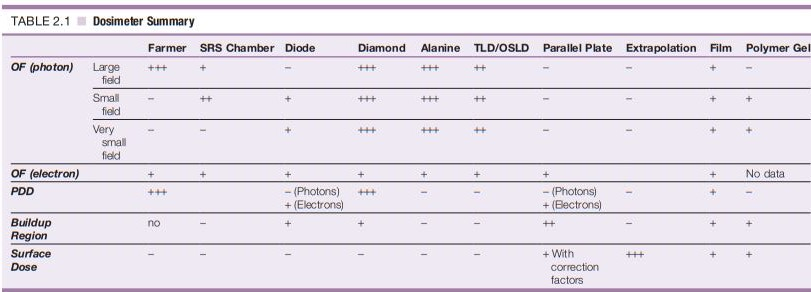
\includegraphics[width=1.0\textwidth]{Imagens/dosimetrosDosimetriaRelativa.JPG}
		}%
		\caption{Dosímetros aplicados em dosimetria relativa.}
		\label{fig:dosimetrosDosimetriaRelativa}
	\end{figure}


\section{Prática Recomendada para Varredura do Feixe}

	Os dados brutos do feixe contêm artefatos criados por ondulações na água causadas pelo detector/movimento mecânico próximo à superfície, ruído do detector e incertezas mecânicas. O processamento de dados do feixe destina-se a remover esses artefatos. Como o processamento de dados, como a suavização e tornar os dados simétricos, pode, por sua vez, introduzir incertezas, é uma prática recomendada manter o processamento no mínimo necessário.

	Para todas as medidas, o gantry deve estar nivelado com a superfície da água antes de realiza-las. A máquina é alinhada o mais verticalmente possível, primeiro usando uma ``escala'' e, em seguida, indicadores CAX de feixe do Gantry, se disponíveis. Na próxima etapa, o alinhamento do CAX é verificado pela varredura de perfis de feixe ``cruzado'' (\textit{cross-beam profiles}) em duas profundidades diferentes (por exemplo, 5 cm e 30 cm). Os softwares modernos de scanner de água geralmente possuem uma ferramenta integrada para a verificação vertical do CAX. A \ref{fig:scanningArmTilt} demonstra os efeitos da inclinação do braço de escaneamento no levantamento dos perfis do feixe, que ocorre quando o tanque não é alinhado corretamente.

	\begin{figure}[h]
		\centering
		\fcolorbox{DarkTurquoise}{white}{%
			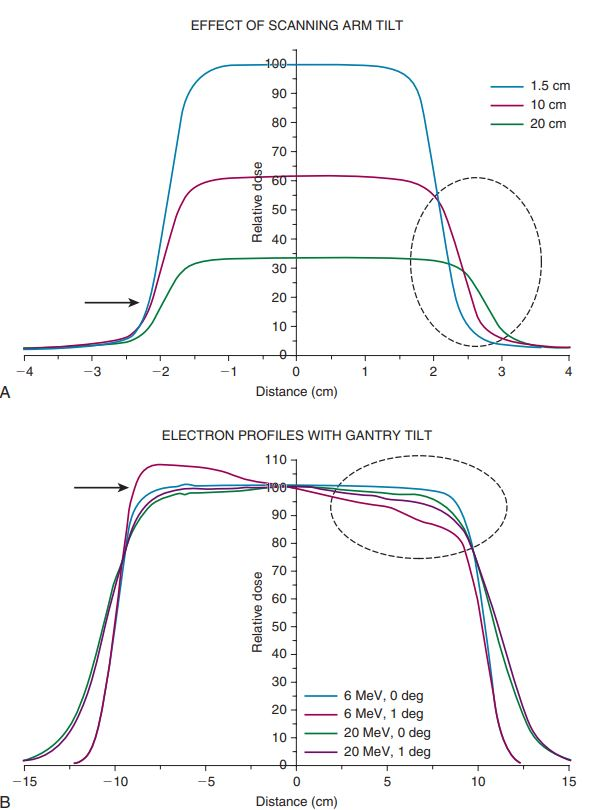
\includegraphics[width=0.5\textwidth]{Imagens/scanningArmTilt.JPG}
		}%
		\caption{Efeitos da inclinação do braço de varredura nos dados do perfil do feixe.}
		\label{fig:scanningArmTilt}
	\end{figure}

	Para definir a posição da superfície usando a reflexão do detector na superfície da água, é importante mover o detector em direção à superfície da água por baixo para minimizar o efeito da tensão superficial. Uma gota de sabão líquido ou detergente pode ajudar a minimizar a tensão da água. Ao coletar dados de feixe em um período de tempo estendido, como os dias ou semanas necessários para o comissionamento, a evaporação da água não é desprezível e pode chegar a 1 mm/dia. Portanto, é necessário verificar a configuração pelo menos diariamente para verificar se a superfície da água, a distância da fonte à superfície (SSD) e outros parâmetros relativos à superfície da água ainda estão dentro dos níveis de tolerância desejados. A \ref{fig:posicaoDetector} mostra como usar a reflexão do detector na superfície da água para definir a posição correta da superfície. É essencial abordar a superfície da água por baixo para minimizar o efeito da tensão superficial.

	\begin{figure}[h]
		\centering
		\fcolorbox{DarkTurquoise}{white}{%
			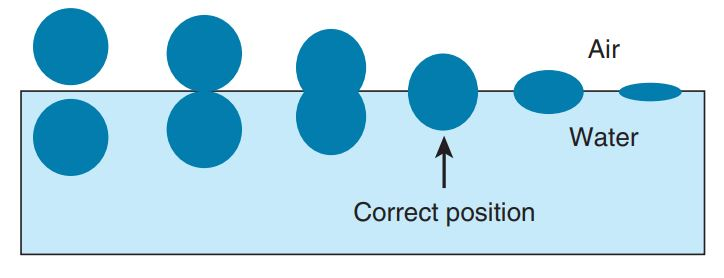
\includegraphics[width=0.5\textwidth]{Imagens/posicaoDetector.JPG}
		}%
		\caption{Posição correta do detector na superfície da água.}
		\label{fig:posicaoDetector}
	\end{figure}

	Em resumo, a ordem da configuração do tanque de água e do detector deve ser:

	\begin{enumerate}[label=\textcolor{CarnationPink}{\arabic*${}^\circ $}]
		\item Alinhar cuidadosamente o phantom de água e o gantry do feixe um com o outro. Os eixos do movimento do phantom de água devem estar alinhados com os eixos x e y do acelerador (em coordenadas IEC). O acelerador deve estar em 0 graus com a maior precisão possível.
		
		\item Verificar a precisão dos parâmetros de setup várias vezes, especialmente se for necessário um tempo prolongado de aquisição de dados em um tanque de água. A evaporação pode alterar a localização da superfície da água na ordem de 1 mm ou mais por dia.
		
		\item Configurar e nivelar com precisão o tanque de água e os eixos mecânicos de movimento.
		
		\item Definir cuidadosamente os locais para superfície da água, eixo central do feixe e correção vertical CAX.
		
		\item Usar o comprimento mínimo possível de cabo no feixe.
		
		\item Definir a velocidade de varredura de modo que a perturbação da superfície da água seja mínima, especialmente em baixas profundidades de varredura para aquisição de OARs.
		
		\item Ajuste a velocidade de varredura para a taxa de dose de modo que uma boa relação sinal-ruído do detector esteja presente nos locais de baixo sinal do feixe (por exemplo, PDP em profundidade, região além da penumbra para OAR).
		
		\item Defina o espaçamento do ponto de dados de varredura pequeno o suficiente para medir com precisão as regiões de alto gradiente no feixe;
	\end{enumerate}

	A técnica de varredura também influencia a qualidade dos dados na região da penumbra. Para melhores resultados, os seguintes parâmetros de varredura devem ser definidos para a região de penumbra:

	\begin{itemize}[label=\textcolor{CarnationPink}{$\star$}]
		\item A velocidade de varredura deve ser lenta o suficiente para permitir uma relação sinal-ruído adequada em toda a faixa de taxas de dose na região da penumbra.
		\item Os pontos de dados de varredura devem ser espaçados de perto para definir bem os ombros e o ponto de inversão (usado para determinação de FWHM);
		\item A varredura deve ser estendida de 5 a 10 centímetros além da penumbra.
	\end{itemize}


\section{Medidas de Dosimetria Relativa}

\subsection*{Posicionamento do Detector de Referência}

	Para medida de PDP, OAR e algumas TPR, um detector de referência deve ser utilizada para eliminar incertezas causadas pela instabilidade no output do feixe durante o tempo de aquisição de dados. Embora o TG-106 ainda recomende o uso de um detector de referência, os linacs mais modernos alcançaram estabilidade no outupt boa o suficiente para garantir que  dados de referência de boa qualidade possam ser adquiridos sem o uso de um detector de referência, porém até que os dados publicados a respeito da não utilização de câmaras de referência estejam disponíveis, a melhor prática permanece a utilização de um detector de referência. Existem quatro locais possíveis para colocar um detector de referência, conforme mostrado na \ref{fig:posicaoDetector}. A posição tradicional é dentro do campo medido conforme mostrado para o Detector de referência 2, ou no ar ou na água em direção à superfície do phantom de água. Para campos pequenos, esta posição pode introduzir perturbação do campo ou ``sombreamento'' no campo do detector, o que é especialmente uma preocupação para medidas de OAR. A melhor alternativa é colocar o detector de referência em uma posição dedicada acima dos colimadores secundários, conforme mostrado para o Detector de referência 1, o que requer que o cabeçote Linac seja projetado para fornecer um espaço para um detector de referência. Uma boa alternativa ,se o acesso à cabeça do acelerador não estiver disponível, é colocar o detector de referência no fundo do tanque de água abaixo do detector de campo, conforme mostrado para o Detector de Referência 4. A divergência do campo cria uma seção transversal de feixe maior no qual permite colocar o detector de referência com mais facilidade para evitar a sobreposição do detector com o campo ou a perturbação no campo em comparação com a posição do Detector de referência 2. O TG-106 declara especificamente que um detector de referência não deve ser colocado fora do feixe primário (Detetor de referência 3) porque a baixa quantidade de espalhamento levaria a uma baixa relação sinal-ruído para o detector de referência. A quantidade de cabo do detector no feixe deve ser minimizada tanto quanto possível.

	\begin{figure}[h]
		\centering
		\fcolorbox{DarkTurquoise}{white}{%
			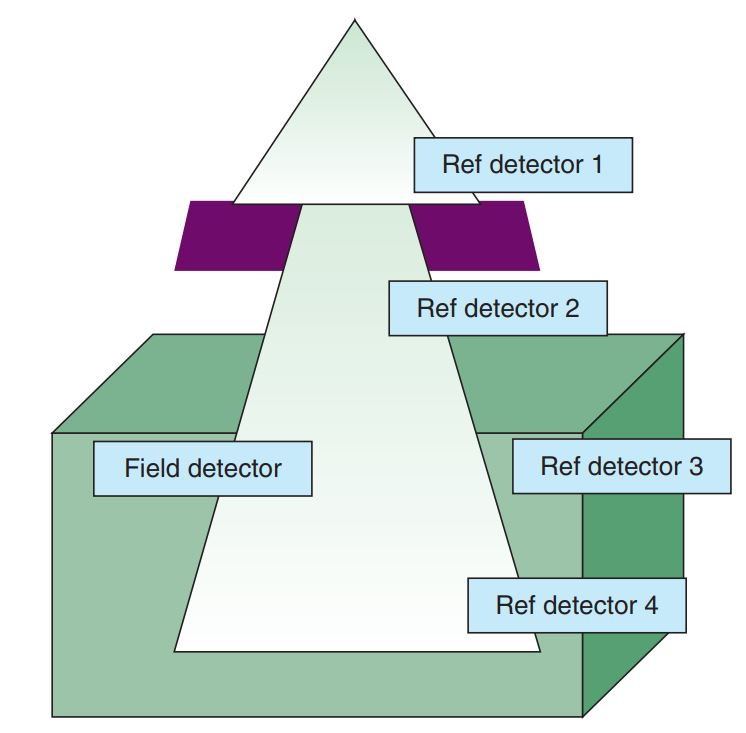
\includegraphics[width=0.8\textwidth]{Imagens/locaisDetectoresReferencia.JPG}
		}%
		\caption{Possíveis localizações do detector de referência: (1) acima dos colimadores secundários, (2) no campo, (3) fora do campo, (4) na parte inferior do campo.}
		\label{fig:posicaoDetector}
	\end{figure}

	\begin{tcolorbox}[width=\textwidth, colback={white}, colbacktitle={DarkTurquoise!50!white}, title={$\bigstar$ \LobsterTwo{Nota: Razão Sinal-Ruído} $\bigstar $}, coltitle={CarnationPink}, colframe={DarkTurquoise}, fonttitle=\rmfamily\bfseries\Large]
		$\quad$ A razão sinal-ruído (também conhecida como SNR, do inglês "Signal-to-Noise Ratio") é uma medida que descreve a relação entre o sinal desejado e o ruído indesejado em um determinado sistema ou sinal. O sinal refere-se à parte útil ou desejada de um sistema ou sinal, enquanto o ruído representa as interferências, distorções ou componentes indesejados que afetam a qualidade ou a fidelidade do sinal.

		$\quad$ A razão sinal-ruído é expressa como a relação entre a potência ou amplitude do sinal e a potência ou amplitude do ruído na maior parte dos sistemas de comunicação e sinais. No entanto, quando se trata de detectores de radiação, os parâmetros que determinam a razão-ruído podem mudar dependendo das características específicas do detector e do tipo de radiação sendo detectada. A razão sinal-ruído em detectores de radiação geralmente envolve parâmetros específicos, como eficiência quântica, ganho, tempo de aquisição, limite de detecção e níveis de ruído eletrônico. 

		$\quad$ Em muitos casos, a razão sinal-ruído em detectores de radiação é expressa como uma relação entre o sinal de interesse (por exemplo, número de eventos detectados) e o ruído de fundo (por exemplo, eventos aleatórios, ruído eletrônico).
	\end{tcolorbox}

	A direção da varredura é importante. Para levantamentos de PDP, é melhor fazer a aquisição dos dados iniciando na maior profundidade até a superfície para minimizar os efeitos da tensão da água. Levantamentos de perfil normalmente devem ser adquiridos utilizando a dimensão de resolução mais alta do detector (a exceção é para diodos em que os efeitos de dependência angular determinam que o diodo seja irradiado “end on”). Isso aumentará o tempo de aquisição, mas produzirá dados mais precisos, se necessário.

\subsection*{Fator de Output na água (Fator de Espalhamento Total)}

	O OF ou fator de espalhamento total ($S_{c,p}$) é definido como a taxa de output para o tamanho do campo x, normalizado para o tamanho do campo de referência. Na maioria dos aceleradores, o tamanho do campo de referência é 10 cm x 10 cm; o campo de referência específico da máquina é usado em dosimetria de campos pequenos.

	Para medir o fator de output, o detector precisa estar centralizado no CAX do feixe de radiação. O procedimento clínico é primeiro alinhar visualmente o centro do detector com o  laser CAX ou o retículo do campo de luminoso. Como a tolerância dos indicadores ópticos  ao CAX do feixe é $<$ 1 mm e o volume ativo do detector pode variar ligeiramente dentro do invólucro do detector, esse alinhamento visual deve ser ajustado usando varreduras de perfil transversal. A maioria dos phantoms de água tem a funcionalidade de realizar varreduras de perfil transversal, determinar o CAX do feixe em cada direção e deslocar o detector para o CAX do feixe medido. O ajuste de posição CAX do detector baseado em varredura de perfil transversal deve ser iterado até que o detector esteja posicionado dentro de 0,1 mm do CAX do feixe.

	Para a escolha do detector utilizado para medir os fatores de output, várias características físicas do feixe devem ser consideradas. O espectro de energia do feixe muda conforme o tamanho do campo muda. Portanto, a resposta do detector deve ter baixa dependência energética. O menor tamanho de campo a ser medido determina as dimensões máximas do detector que podem ser usadas sem introduzir erros devido à média de volume no centro do campo. Este efeito é ainda mais importante para medidas de OF em feixes pequenos FFF.

	Existem várias abordagens possíveis para medidas do OF em uma ampla gama de tamanhos de feixe. Normalmente, um detector como uma câmara do tipo Farmer ou outra câmara de ionização é usado para medir o OF desde o tamanho máximo do campo até um tamanho mínimo do campo de cerca de 4 cm x 4 cm. Abaixo desse tamanho de campo, detectores menores, como câmaras de ionização de volume pequeno, diodos ou detectores de diamante, oferecem o menor tamanho de detector necessário para medidas de campos pequenos. O tamanho do campo de 4 cm x 4 cm é uma boa escolha para calibração cruzada do OF medido dos campos grandes com as medições dos campos pequenos, uma vez que a mudança de energia do campo de 4 cm x 4 cm para o o menor tamanho de campo é minimizado se forem usados diodos. As câmaras de ionização de pequeno volume, por outro lado, podem não ser adequadas para medidas do OF em grandes campos, porque a proporção da haste irradiada para o volume do detector é grande. Para campos muito pequenos (isto é, campos abaixo de 2 cm x 2 cm de tamanho de campo), o espectro de energia muda significativamente o suficiente para afetar a resposta de energia tanto das câmaras quanto dos diodos. Isso levou a estudos com simulação de Monte Carlo e comparações com o OF medido com gel para determinar fatores de correção para resposta do detector nas condições de irradiação de campos pequenos. O TG-155 sobre dosimetria de pequenos campos e o Grupo de Trabalho da IAEA sobre dosimetria de pequenos campos possuem documentos para revisar os fatores de correção de detectores publicados e oferecer recomendações.

	Os fatores de output de elétrons são definidos como a razão da dose por MU na profundidade $d_{max}$ para o campo medido e a dose por MU em $d_{max}$ para o campo de referência. O campo de referência é normalmente escolhido para ser o cone aberto de 10 cm x 10 cm. Como $d_{max}$ para  os elétrons muda em função do tamanho do campo, tornando-se mais raso à medida que o campo diminui e atinge a faixa de equilíbrio eletrônico, a PDP para campos de elétrons menores deve ser adquirida afim de determinar a profundidade para medir o OF.

	Os OF de elétrons são normalmente medidos no comissionamento para todas as energias, todos os cones abertos disponíveis, todos os recortes (cutouts) clínicos padrão quadrados e circulares e para as SSDs de 100 cm, 105 cm e 110 cm. O TPS com recursos de MC para elétrons podem exigir medidas adicionais de OF. Para cutouts personalizados que são relativamente próximos em forma de recortes padrão retangulares ou quadrados, o OF pode ser interpolado usando modelos computacionais baseados em medidas de PDP e OF de campos convencionais. 

	O TG-25 aborda métodos computacionais básicos, enquanto TG-70 discute os desenvolvimentos mais recentes, incluindo as incertezas dos modelos de cálculo do OF. Para blocos de elétrons personalizados muito irregulares, o OF deve ser medido por paciente se as formas de campo diferirem muito das formas de recorte padrão que os modelos computacionais não podem ser aplicados. Além disso, a profundidade de $d_{max}$ deve ser verificada. Como a irregularidade não pode ser facilmente quantificada, na prática clínica é comum medir uma variedade de formas de recorte de pacientes individuais até que uma biblioteca personalizada seja desenvolvida para fornecer uma variedade de dados para comparação.

	Ocasionalmente, os campos de elétrons precisam ser moldados de modo que o eixo central seja bloqueado. Para esses campos, o detector deve ser colocado no centro da seção de campo aberto do cutout. Para campos muito irregulares (por exemplo, campos com uma grande área aberta e uma longa seção estreita), pelo menos dois conjuntos de medidas devem ser feitos: no centro da grande área aberta e na área estreita. O filme radiográfico/radiocrômico também pode ser usado para obter um gráfico 2D da variação de dose em toda a área do campo. É então uma decisão clínica do médico de como ajustar o MU para obter a distribuição de dose desejada para o paciente. A \ref{fig:locaisDetectoresEletrons} mostra exemplos de uma forma de campo com bloqueio do eixo central e uma forma de campo altamente irregular.

	\begin{figure}[h]
		\centering
		\fcolorbox{DarkTurquoise}{white}{%
			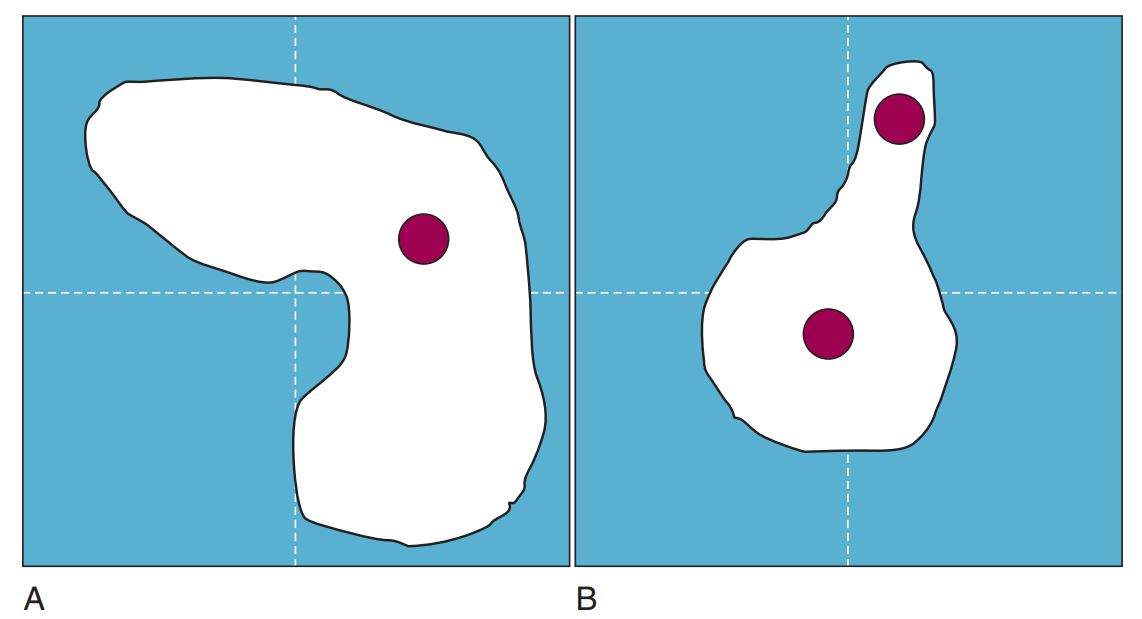
\includegraphics[width=0.5\textwidth]{Imagens/locaisDetectoresEletrons.JPG}
		}%
		\caption{Exemplo de localizações de detectores para medidas do fator de output (OF) dos feixes de elétrons em recortes irregulares. \textcolor{MediumOrchid}{\textbf{A}} mostra um grande recorte com o eixo central bloqueado. O OF deve ser medido no centro aproximado do campo. \textcolor{MediumOrchid}{\textbf{B}} mostra um campo altamente irregular. O OF deve ser medido no centro do setor aberto e uma segunda medida deve ser feita na seção estreita para avaliar a mudança no OF.}
		\label{fig:locaisDetectoresEletrons}
	\end{figure}


	O TG-70 que estabelece um protocolo de dosimetria de feixe de elétrons fornece uma regra prática para quando os campos de elétrons são muito pequenos/estreitos. Uma medida personalizada deve ser feita se:

		\begin{equation}
			raio \; do \; campo \leq 0.88 \sqrt{\bar{E}_0} \; cm
		\end{equation}

	\begin{exemplo}[onde:]
		\begin{itemize}[label=\textcolor{CarnationPink}{$\star$}]
			\item \textcolor{DarkTurquoise}{$\bar{E}_0$} é a energia média do feixe incidente na superfície do phantom;
		\end{itemize}
	\end{exemplo}

	\begin{figure}[h]
		\centering
		\fcolorbox{DarkTurquoise}{white}{%
			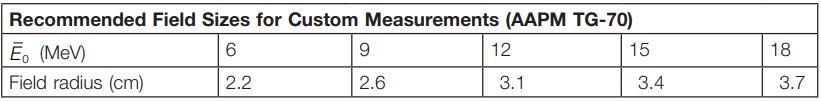
\includegraphics[width=0.9\textwidth]{Imagens/tamanhosDeCampoOFeletrons.JPG}
		}%
	\end{figure}

\subsection*{Fator de Output no Ar (Fator de Espalhamento do Colimador)}

	O fator de output no ar para feixes de fótons, às vezes também chamado de “fator de espalhamento do colimador ($S_c$)”, é utilizado em alguns modelos de feixe para modelar melhor as diferentes contribuições da dose espalhada nos modelos computacionais de cálculo de dose. 

	O TG-74 fornece uma discussão detalhada sobre a base teórica sobre os OFs no ar e desenvolve um protocolo para padronizar as técnicas de medida do output no ar entre as instituições. Tradicionalmente, as capas de buildup têm sido utilizadas para aumentar a espessura da parede do detector para $d_{max}$ para fornecer o equilíbrio eletrônico. No entanto, esse método não evita a contaminação por partículas carregadas para feixes de fótons de altas energias. O TG-74 discute em detalhes os vários mini-phantoms e capas de metal (brass) que foram desenvolvidos para encontrar a geometria ideal para gerar equilíbrio eletrônico enquanto remove a contaminação por partículas carregadas. No entanto, alguns sistemas de planejamento ainda utilizam o método original de medir o OF no ar com capas de buildup para fornecer a espessura igual a $d_{max}$ para realizar cálculos de MU baseados em TMR. Portanto, os físicos médicos devem ter atenção às instruções do manual do TPS para determinar qual configuração experimental é necessária para seu respectivo TPS.

\subsection*{Fator Filto e Perfis}

	As técnicas de aquisição de dados de dosimetria para filtros dependem do tipo de filtro avaliado. Para filtros físicos e filtros universais, os OARs são medidos usando as mesmas técnicas utilizadas nos campos abertos. Os perfis são medidos ao longo da direção do filtro, bem como nos eixos centrais. A medida transversal é recomendada porque o aumento da incidência angular do feixe de radiação filtro para grandes campos pode causar “arredondamento” do perfil transversal do filtro. Para medir o fator de transmissão do filtro, o detector é posicionado no eixo central e dois conjuntos de medidas são realizados onde o filtro é girado em 180 graus entre as medidas. Esta técnica reduz as incertezas introduzidas pela imprecisão no alinhamento do detector com o CAX do filtro.

\subsection*{PDP}

	Para medir a PDP em feixes  FFF, campos pequenos ou campos muito pequenos, é essencial alinhar o CAX feixe dentro de $<$ \ang{0.5} e usar a função de correção de CAX do phantom de água.  Um desalinhamento do feixe de \ang{0.5} em relação ao movimento vertical do detector causará um desvio do detector em relação ao CAX do feixe de 0.9 mm a 10 cm de profundidade. Como campos pequenos FFF ou campos muito pequenos consistem predominantemente em penumbra, mesmo um pequeno desalinhamento do CAX do detector com o CAX do feixe pode levar a erros na PDP de 5\% ou mais. Uma PDP desalinhada mostrará uma queda de dose mais acentuada na profundidade em comparação com os dados padrão. Como o feixe endurece com a profundidade, as medidas de PDP em campos pequenos devem ser realizadas com detectores que tenham baixa dependência de energia.

	O TG-51 recomenda um deslocamento da curva PDP de $0.6 \cdot r_{cav}$ para feixes de fótons e $0.5 \cdot r_{cav}$ para feixes de elétrons quando a PDP é medida com câmaras cilíndricas ou esféricas. Nenhum deslocamento é necessário para medidas de PDP utilizando diodos ou câmara de placas paralelas, porque não há divergência de feixe significativa ao longo da profundidade da câmara ao deslocar o ponto efetivo de medida. Para feixes de elétrons, a curva de ionização na profundidade deve ser convertida em uma curva de dose na profundidade através da aplicação das razões de poder de freamento adequadas (que são dependentes da profundidade). A maioria dos scanners de tanques de água comerciais possuem algoritmos automáticos para realizar essa correção, que não é necessária caso for utilizado diodos.

	Técnicas experimentais especiais são necessárias para medir com precisão a dose superficial e a PDP para a região de buildup. Na prática clínica, geralmente é bem entendido que a dose superficial exibida pelo TPS carrega uma grande incerteza. Para situações clínicas em que é necessária uma dose precisa em estruturas superficiais, o bolus é normalmente utilizado para mudar a distribuição da dose em direção à superfície da pele. Além de aumentar a dose na pele, isso também traz  mais precisão na da PDP em direção à superfície da pele. A exceção a esta regra  são os pacientes de cabeça e pescoço, onde tanto alvos clínicos quanto estruturas críticas podem ser encontrados próximos à superfície da pele. Como a dose para essas estruturas superficiais é uma combinação do feixe anterior, da dose devido a saída dos feixes contralaterais e da dose das bordas dos campos das demais incidências, a dose absoluta originada da região de buildup de um feixe que contribui para dose mais superficial é relativamente pequena. A energia do feixe usada para pacientes de cabeça e pescoço, bem como para pacientes nos quais o bolus é usado, é tipicamente o feixe de fótons de menor energia (ou seja, 6 MV na maioria dos casos). Portanto, se um físico deseja realizar uma medida de dose superficial e da região de buildup com  maior precisão com um detector diferente daquele usado para determinar a PDP além do $d_{max}$, o feixe de 6 MV seria a melhor escolha em relação ao impacto clínico devido à melhoria da precisão desses feixes.

	Idealmente, a dose de superfície seria medida com uma câmara de extrapolação. A disponibilidade do detector e o tempo de medição geralmente limitam esta opção, especialmente devido à relativa significância clínica. A melhor alternativa ao uso de uma câmara de extrapolação são as câmaras de placas paralelas com uma pequena separação de placas, janela de entrada fina e anel de guarda largo. A região de buildup é caracterizada por um gradiente de dose acentuado, falta de equilíbrio eletrônico e componente de baixa energia do feixe relativamente alta. Como sempre, para medidas em gradientes de dose acentuado, o uso de um detector com uma dimensão pequena na direção do gradiente melhorará a precisão das medidas. A direção de levantamento da PDP na região de buildup deve ser sempre iniciada em $d_{max}$ em direção à superfície da água para evitar problemas causados pela tensão superficial da água.

	Para medidas da PDP, a ordem do setup é:

	\begin{enumerate}[label=\textcolor{CarnationPink}{\arabic*${}^\circ $}]
		\item Alinhamento vertical do feixe de radiação usando indicadores de CAX ópticos e/ou níveis mecânicos;
		\item Alinhamento do phantom  de água: alinhamento geral do tanque seguido pelo alinhamento dos eixos mecânicos à superfície da água;
		\item Varreduras de perfil transversal para definir a posição zero do detector no CAX do feixe na profundidade;
		\item Varreduras de perfil transversal em duas profundidades (por exemplo, $d_{max}$ e 20 cm) para determinar o ângulo do CAX;
		\item Medir a PDP;
		\item Se desejado, as medidas de PDP são seguidas por medidas dedicadas de dose superficial e da PDP da região de buildup para as energias selecionadas;
	\end{enumerate}

	De acordo com as recomendações TG-70 para dosimetria de feixe de elétrons, o padrão-ouro para medir a PDp para elétrons é uma câmara de ionização (placas paralelas ou cilíndricas) em um phantom de água. A PDP é estabelecida medindo-se a curva de percentual de ionização na profundidade e, para câmaras de ionização cilíndricas, convertendo-a em uma curva de PDP usando as equações descritas na parte de dosimetria de referência. 
	
	As PDPs de elétrons também podem ser medidos diretamente utilizando diodos para elétrons, filmes ou detectores de diamante. Esses detectores devem ser primeiramente verificados em relação às PDPs medidas com câmaras de ionização para verificar se a resposta do detector leva a resultados de PDP comparáveis. O TG-70 fornece instruções detalhadas sobre a medida precisa da PDP usando câmaras de ionização; o O TG-25 abrange medidas de PDP utilizando diodos. O filme é um dosímetro muito útil para medidas de PDP em campos irregulares. O filme é alinhado em um phantom de água sólida com o filme paralelo ao feixe e a borda do filme orientada ao longo da menor dimensão do campo. Além da PDP, o resultado da medida também fornecerá as curvas de isodose. Para campos correspondentes (match), o filme pode fornecer informações da PDP, bem como informações sobre a sobreposição de dose na região de correspondência.
	
	A maioria dos TPSs requerem dados da PDP do feixe, com exceção do TPS dedicado para SRS limitados a campos pequenos. A razão para esta exceção é que medir a PDP com precisão é cada vez mais difícil para tamanhos de campo pequenos, especialmente em feixes FFF, porque requer que o detector se desloque com precisão no CAX do feixe de radiação na profundidade com uma tolerância $<$ 0.2 mm em toda a faixa de medida na profundidade. Devido a essa grande incerteza na medição de PDD para campos pequenos, os físicos não devem tentar medir a PDP e depois trabalhar os dados do feixe usando uma conversão de PDP para TPR. Embora esse método possa ser aceitável para tamanhos de campo grandes, ele introduzirá grande incerteza nos dados do TPR.

	A medida de dados de TPR em um phantom de água em um linac é um desafio, porque requer o deslocamento do tanque de água e do detector com muita precisão. Portanto, as medidas de TPR geralmente são feitas em placas menores (ou seja, mais leves) de material água-equivalente colocadas na mesa de tratamento. As medidas de TPR para o CyberKnife são realizadas montando o detector em uma estrutura fixada ao cabeçote do linac; o linac pode então ser conduzido verticalmente para cima e para baixo usando o robô para alterar a profundidade do detector na água. Nos últimos anos, pequenos phantoms de água direcionados para medidas de TPR para SRS tornaram-se disponíveis para tornar as medições da TPR mais eficientes. Outra solução é usar caixas d'água onde a água pode ser bombeada para dentro ou para fora da caixa automaticamente; um sensor que mede a posição da superfície da água pode fornecer a profundidade da TPR.

\subsection*{Razão Off-Axis (OAR)}

	As razões Off-Axis (OARs), ou perfis do feixe, são tomadas em várias profundidades para caracterizar o perfil do feixe. Para campos quadrados, retangulares e circulares, geralmente são usadas duas OARs em um ângulo de 90 graus. Outras formas de feixe (por exemplo, o feixe hexagonal criado pelo colimador IRIS do CyberKnife) requerem mais perfis de feixe em ângulos determinados pelo colimador. O TG-106 recomenda que os dados obtidos NÃO sejam dimensionados para fornecer valores em diferentes SSDs necessárias nos sistemas de planejamento. Isso ocorre porque um maior tamanho de campo projetado altera as condições de espalhamento e a contaminação com elétrons é diferente em diferentes SSDs. Esta recomendação não se aplica a sistemas de planejamento de tratamento que exigem que os OARs sejam medidos em condições de TPR.

	A parte mais importante do perfil OAR é a região de penumbra definida pelas isodoses de 20\% a 80\%, porque esta região fornece o gradiente de dose íngreme usado para tratamentos de IMRT e SBRT. A região da penumbra tem várias características dosimétricas principais como gradiente de dose acentuado, grande mudança na taxa de dose, mudança na energia do feixe e falta de equilíbrio eletrônico lateral. A escolha do detector deve, portanto, ser focada em pequenos detectores com baixa dependência com a taxa de dose e com baixa dependência energética.

	Mesmo usando excelentes práticas de aquisição de dados, algum processamento de dados ainda será necessário. Geralmente isso engloba:

	\begin{itemize}[label=\textcolor{CarnationPink}{$\blacktriangleright$}]
		\item Suavização dos dados para minimizar o ruído; deve-se ter cuidado na escolha dos parâmetros de suavização para manter a forma dos altos gradientes dose na região da penumbra.
		\item Tornar os OARs simétricos; isso reduz os erros introduzidos pelo ponto de medida efetivo do detector versus o alinhamento CAX do feixe ou assimetria do colimador.
		\item Somente para campos circulares, deve-se obter a média de OARs in-line e cross-line; Isso não deve ser feito para campos quadrados, porque a penumbra em particular pode ser diferente devido às diferenças mecânicas nos colimadores que definem os lados dos campos.
	\end{itemize}

\section{Considerações de Segurança}

	Um recurso de segurança essencial é a revisão por pares dos dados de dosimetria relativa. O TG-103, Revisão por Pares em Física de Radio-Oncologia, fornece diretrizes sobre revisão por pares entre dois físicos da radioterapia; O Código de Ética TG-109 abrange os aspectos éticos do processo de revisão por pares.

	Para facilitar um processo eficaz de revisão por pares, o relatório de comissionamento deve ser preenchido e disponibilizado ao físico responsável pela revisão. O relatório de comissionamento deve conter comparações dos conjuntos de dados adquiridos com conjuntos de dados padrão publicados. Quaisquer desvios dos dados publicados em mais de 3\% devem ser minuciosamente investigados. O conjunto completo de dados de dosimetria relativa deve ser claramente rotulado e salvo em um local disponível para todos os físicos e pode ser disponibilizado para indivíduos ou organizações envolvidas na revisão por pares. Os dados devem ser protegidos contra alterações/modificações acidentais ou intencionais e devem ter backup de segurança.

\bibliography{ref.bib}
\end{document}